% =====================================================================
%  Milestone 4 — Generalisation Across Generator Families
%  % =====================================================================
%  Milestone 4 — Generalisation Across Generator Families
%  % =====================================================================
%  Milestone 4 — Generalisation Across Generator Families
%  % =====================================================================
%  Milestone 4 — Generalisation Across Generator Families
%  \input{chapters/ch_milestone4}
% =====================================================================
\chapter{Milestone 4 --- Generalisation Across Generator Families}
\label{ch:milestone4}

\section{Motivation}

Every result in Chapters~\ref{ch:results} and~\ref{ch:rejected} is measured on one
generator family: Qwen2.5-Coder, at 1.5B, 7B and 32B parameters. The scale sweep
shows that the specification gap and the flat spatial accuracy persist across that
range, which rules out capacity \emph{within} the Qwen family as an explanation. It
does not rule out the family itself. A reader can reasonably ask whether the released
prompt's failure is a property of ViperGPT's specification or a property of how one
vendor's models happen to follow instructions --- and, separately, whether a stronger
publicly available generator narrows the gap to the paper's reported $72.0$.

This chapter answers both with a second, orthogonal sweep: four model families across
all four prompt conditions on both datasets.

\section{Design}

\begin{table}[htbp]\centering\small
\caption{The four generators. All are openly downloadable without licence acceptance
or an access token, so the grid is reproducible without credential management --- a
deliberate choice, given that the dissertation's subject is a system rendered
irreproducible by a withdrawn proprietary model.}
\label{tab:m4-models}
\begin{tabular}{@{}llll@{}}
\toprule
\textbf{Generator} & \textbf{Publisher} & \textbf{Parameters} & \textbf{Note} \\
\midrule
Qwen2.5-Coder-7B-Instruct & Alibaba & 7B dense & used throughout Ch.~\ref{ch:results} \\
DeepSeek-Coder-V2-Lite-Instruct & DeepSeek & 16B / \textbf{2.4B active} & mixture-of-experts \\
Yi-Coder-9B-Chat & 01.AI & 9B dense & --- \\
OpenCoder-8B-Instruct & INF / M-A-P & 8B dense & needs \texttt{trust\_remote\_code} (D15) \\
\bottomrule
\end{tabular}
\end{table}

Each model was run under all four prompt conditions (C1--C4,
Section~\ref{sec:prompts}) on both datasets at $n=500$ with greedy decoding --- the
same protocol as every other result in this dissertation. Combined with the existing
Qwen-7B cells this gives a $4 \times 4 \times 2 = 32$-cell grid. Qwen2.5-Coder-1.5B
and -32B contribute C1 and C2 on RefCOCO from the earlier scale sweep and are
included in the C1$\to$C2 analysis only (D18).

\textbf{What the design isolates.} The prompt conditions are unchanged; only the
generator varies. A difference between models under the same condition is therefore
attributable to the generator, and a difference between conditions that holds across
all four generators is attributable to the prompt rather than to one vendor's
instruction-following.

\textbf{What it does not control for.} DeepSeek-Coder-V2-Lite is a mixture-of-experts
model with 16B total parameters but only 2.4B active per token --- roughly a third of
the smallest dense model here. Any DeepSeek result is confounded by architecture and
effective capacity simultaneously and is reported as such rather than treated as
size-matched. All four generators were released in 2024--2025, two to three years
after Codex, so the grid is not a controlled test of model era.

\section{Engineering}

Three failures occurred while building the grid. Two are general lessons rather than
incidental bugs.

\subsection{A global flag broke the model it was not meant for}

OpenCoder ships custom tokenizer and model classes and requires
\texttt{trust\_remote\_code=True}. Setting the flag globally broke DeepSeek: it forced
\texttt{transformers} to load the repository's own \texttt{modeling\_deepseek.py} in
preference to the library's built-in class, and that file imports
\texttt{is\_torch\_fx\_available}, removed in \texttt{transformers}~5.x.

\begin{lstlisting}[caption={The flag is made conditional on the model identifier
rather than applied uniformly (D15).}]
tok = AutoTokenizer.from_pretrained(
    a.model, padding_side="left",
    trust_remote_code=("OpenCoder" in a.model))
\end{lstlisting}

\subsection{A resumability bug reported failure as success}

The generation script creates its run directory \emph{before} loading the model, so
when the flag above crashed DeepSeek at model-load time, eight empty directories were
left behind. The grid driver's resume logic checked only for the directory's
existence, so the next submission treated all eight as complete, skipped them, and
reported success having generated nothing.

\begin{lstlisting}[caption={Completion is tested by the artefact, not by the
container created to hold it.}]
EXPECT="outputs/runs/*m1_${DS}_testA_${SHORT}_${TAG}_greedy"
if compgen -G "$EXPECT/programs.jsonl" > /dev/null; then
    echo ">>> SKIP  $DS | $PROMPT  (already generated)"
    continue
fi
\end{lstlisting}

This generalises beyond the project: in a resumable pipeline the marker of completion
must be the output artefact, never a side effect of having started.

\subsection{A batching corruption, not a crash}

After both fixes, DeepSeek's RefCOCO/C1 cell generated at batch size 6 --- the setting
used for the other models --- with a parse rate of $0.4\%$ across 500 samples. Not an
error; near-total corruption. Regenerating at batch size 1 (D17) restored the parse
rate to the range seen on the model's other seven cells. The root cause was not fully
diagnosed since a working fix was found, and it is recorded as a fragility of this
particular mixture-of-experts model under batched greedy decoding on this stack rather
than assumed to generalise.

\section{Results}

\begin{table}[htbp]\centering\small
\caption{Accuracy at IoU $\geq 0.5$, greedy, $n=500$ per cell, testA. Conditions as
defined in Table~\ref{tab:conditions}.}
\label{tab:m4-main}
\begin{tabular}{@{}lrrrrrrrr@{}}
\toprule
& \multicolumn{4}{c}{\textbf{RefCOCO}} & \multicolumn{4}{c}{\textbf{RefCOCO+}} \\
\cmidrule(lr){2-5}\cmidrule(lr){6-9}
\textbf{Generator} & C1 & C2 & C3 & C4 & C1 & C2 & C3 & C4 \\
\midrule
Qwen2.5-Coder-7B & 0.00 & 39.20 & 36.40 & 42.00 & 0.00 & 30.80 & 28.00 & 37.60 \\
DeepSeek-V2-Lite & 0.00 & 29.60 & 38.80 & 41.80 & 0.00 & 24.00 & 38.60 & 38.40 \\
OpenCoder-8B & 0.20 & 40.80 & 37.40 & 43.20 & 0.00 & 30.20 & 28.00 & 31.60 \\
Yi-Coder-9B & 3.80 & 43.80 & 39.00 & \textbf{45.40} & 0.80 & 34.40 & 35.60 & \textbf{43.80} \\
\bottomrule
\end{tabular}
\end{table}

\begin{figure}[htbp]\centering
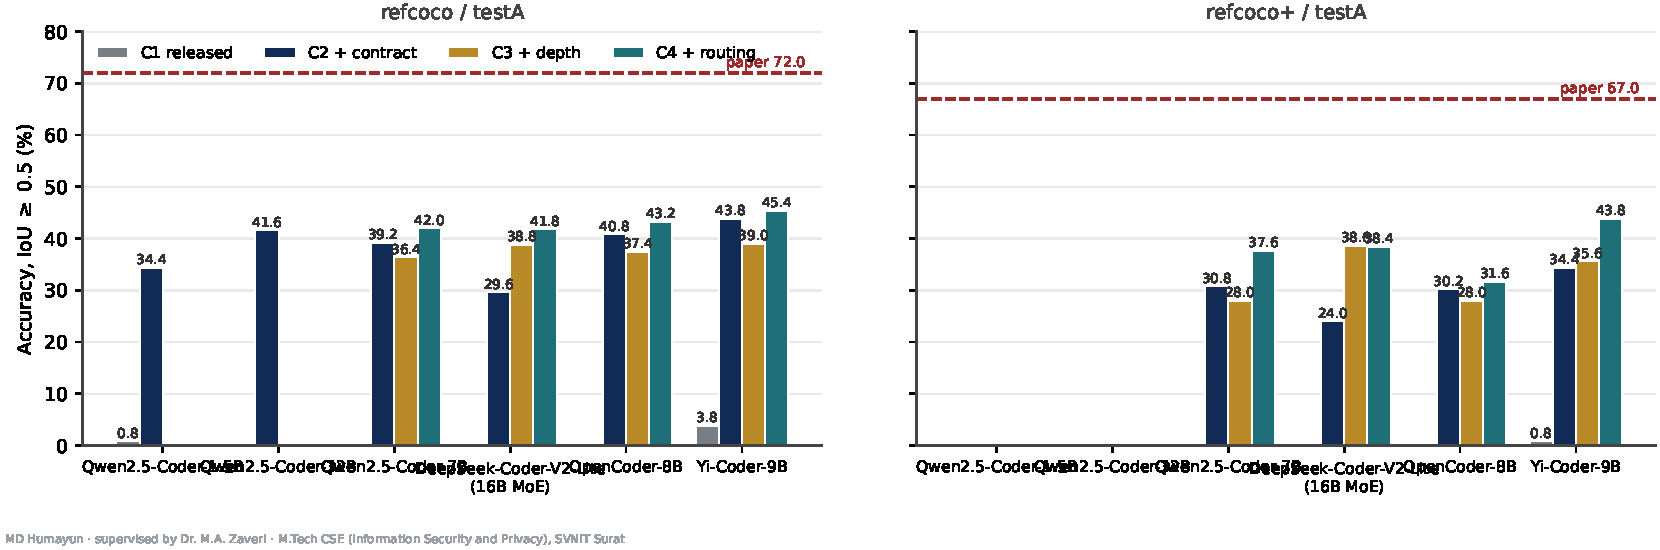
\includegraphics[width=\textwidth]{results/figures/fig17_grid.pdf}
\caption[Accuracy across all generators and conditions]{All four models under all
four conditions, both datasets. The dashed line is the paper's reported figure
($72.0$ on RefCOCO, $67.0$ on RefCOCO+). Every generator is near-zero under C1 and
recovers substantially by C2.}
\label{fig:m4-grid}
\end{figure}

\subsection{Q1 --- is the specification gap universal?}

\begin{table}[htbp]\centering
\caption{C1 $\to$ C2, RefCOCO overall. A gap present in every family cannot be a
property of one model.}
\label{tab:m4-q1}
\begin{tabular}{@{}lrrr@{}}
\toprule
\textbf{Generator} & \textbf{C1} & \textbf{C2} & \textbf{gain} \\
\midrule
Qwen2.5-Coder-1.5B & 0.80 & 34.40 & $+33.6$ \\
Qwen2.5-Coder-7B & 0.00 & 39.20 & $+39.2$ \\
Qwen2.5-Coder-32B & 0.00 & 41.60 & $+41.6$ \\
DeepSeek-V2-Lite & 0.00 & 29.60 & $+29.6$ \\
OpenCoder-8B & 0.20 & 40.80 & $+40.6$ \\
Yi-Coder-9B & 3.80 & 43.80 & $+40.0$ \\
\bottomrule
\end{tabular}
\end{table}

Every generator scores below $4\%$ under the released prompt, and every one recovers
by at least $29.6$ points under the return-type contract alone.
\textbf{The specification gap is not a Qwen-specific failure.} Yi-Coder's baseline of
$3.80$ is the least severe of the six, and it remains a near-total failure relative to
its own $43.80$ under C2.

\subsection{Q2 --- does the depth capability transfer?}

\begin{table}[htbp]\centering
\caption{C2 $\to$ C3 on the RefCOCO+ spatial subset ($n=47$; the depth-word queries).}
\label{tab:m4-q2}
\begin{tabular}{@{}lrrr@{}}
\toprule
\textbf{Generator} & \textbf{C2 spatial} & \textbf{C3 spatial} & \textbf{gain} \\
\midrule
Qwen2.5-Coder-7B & 4.26 & 19.15 & $+14.9$ \\
DeepSeek-V2-Lite & 14.89 & 27.66 & $+12.8$ \\
OpenCoder-8B & 23.40 & 17.02 & $-6.4$ \\
Yi-Coder-9B & 25.53 & 29.79 & $+4.3$ \\
\bottomrule
\end{tabular}
\end{table}

Three of four generators improve on the depth subset when the primitives are offered;
OpenCoder is the exception, losing $6.4$ points.

Two observations matter independently of that exception. First, \textbf{OpenCoder and
Yi-Coder already score far higher than Qwen under C2} --- $23.40$ and $25.53$ against
Qwen's $4.26$ --- \emph{before} any depth primitive is offered. Some generators are
evidently resolving depth relations by other means under the plain grounding contract,
a behaviour not investigated here. Second, Qwen shows both the lowest starting point
and the largest gain, consistent with it benefiting most from an explicit primitive
precisely because it had the least alternative strategy.

At $n=47$ a single query is worth $2.13$ percentage points, so these differences span
roughly two to seven samples. The ordering is informative; the magnitudes are not.

\subsection{Q3 --- is the routing rule necessary in every family?}

\begin{table}[htbp]\centering
\caption{C2 $\to$ C3 $\to$ C4 on the RefCOCO non-spatial subset --- the control
against which over-application of the depth primitives shows up.}
\label{tab:m4-q3}
\begin{tabular}{@{}lrrrrr@{}}
\toprule
\textbf{Generator} & \textbf{C2} & \textbf{C3} & \textbf{C4} & \textbf{C3 change} & \textbf{C4 change} \\
\midrule
Qwen2.5-Coder-7B & 45.97 & 36.02 & 48.82 & $-9.9$ & $+12.8$ \\
DeepSeek-V2-Lite & 31.28 & 45.50 & 50.71 & $+14.2$ & $+5.2$ \\
OpenCoder-8B & 47.87 & 36.49 & 45.97 & $-11.4$ & $+9.5$ \\
Yi-Coder-9B & 49.29 & 49.76 & 52.13 & $+0.5$ & $+2.4$ \\
\bottomrule
\end{tabular}
\end{table}

Two of four generators exhibit the over-application failure that motivated C4 in
Chapter~\ref{ch:results}: Qwen loses $9.9$ points of non-spatial accuracy under C3
and OpenCoder loses $11.4$, and both recover under C4. Yi-Coder does not exhibit it
--- its non-spatial accuracy is flat between C2 and C3 --- yet still gains $2.4$
points from the routing rule.

DeepSeek behaves differently again: its C2 non-spatial accuracy is anomalously low
($31.28$, against $45.97$--$49.29$ for the others), so C3 appears to \emph{gain}
$14.2$ points rather than lose them. This is better read as DeepSeek performing poorly
under C2 than as the depth primitives helping non-spatial queries. Its C2 figures are
the weakest in the grid on both datasets ($29.60$ and $24.00$ overall), which is
consistent with its $2.4$B active parameters.

\textbf{One exception to the C3 $\to$ C4 ordering.} On RefCOCO+, DeepSeek is the sole
generator for which C4 does not exceed C3 ($38.40$ against $38.60$, a $-0.2$
difference). Every other model, and DeepSeek itself on RefCOCO ($38.80 \to 41.80$),
shows $\text{C4} > \text{C3}$. A $0.2$-point difference is one sample in 500 and has
not been re-seeded; it is reported rather than smoothed over, and the claim that C4
improves on C3 is stated as holding in every generator on RefCOCO and in three of four
on RefCOCO+.

\subsection{Q4 --- does a stronger generator raise accuracy?}

\begin{table}[htbp]\centering
\caption{Best condition (C4) against the paper's reported figures.}
\label{tab:m4-q4}
\begin{tabular}{@{}lrrr@{}}
\toprule
\textbf{Generator} & \textbf{C4 RefCOCO} & \textbf{C4 RefCOCO+} & \textbf{share of 72.0 / 67.0} \\
\midrule
Qwen2.5-Coder-7B & 42.00 & 37.60 & 58\% / 56\% \\
DeepSeek-V2-Lite & 41.80 & 38.40 & 58\% / 57\% \\
OpenCoder-8B & 43.20 & 31.60 & 60\% / 47\% \\
Yi-Coder-9B & \textbf{45.40} & \textbf{43.80} & \textbf{63\% / 65\%} \\
\bottomrule
\end{tabular}
\end{table}

\begin{figure}[htbp]\centering
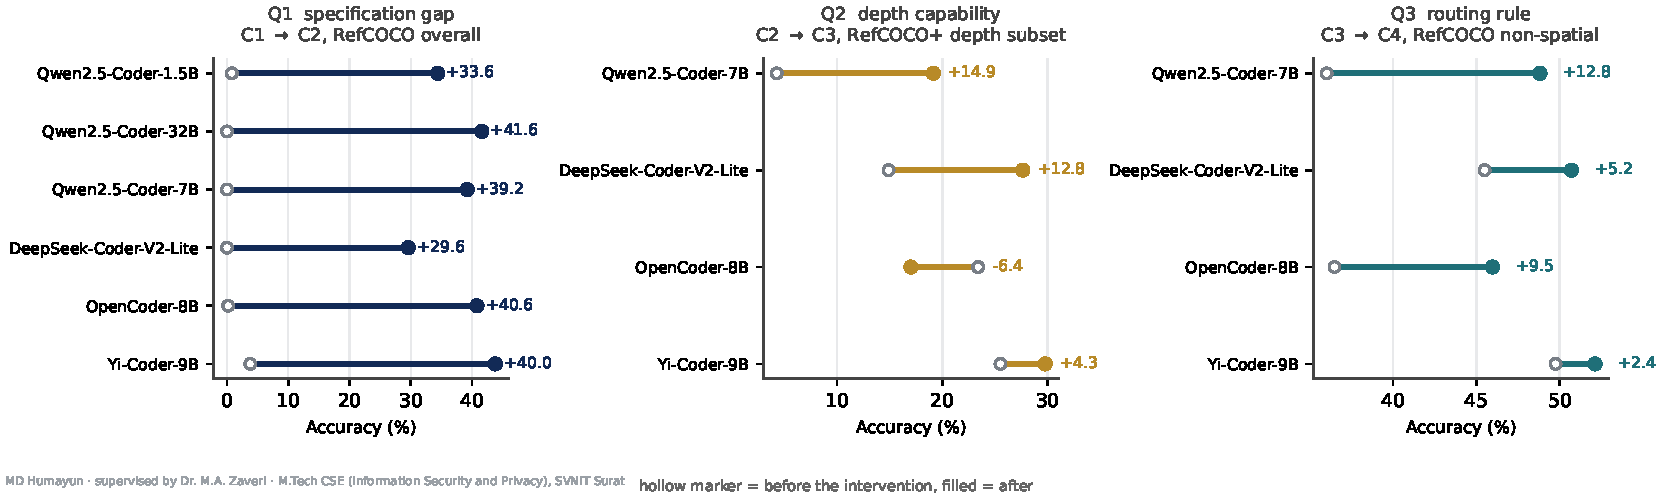
\includegraphics[width=\textwidth]{results/figures/fig18_generalisation.pdf}
\caption[Do the findings transfer across generators?]{Each panel answers one
generalisation question with a before-and-after marker per model: hollow before the
intervention, filled after. Left to right: the specification gap (Q1), the depth
capability (Q2), and the routing rule (Q3).}
\label{fig:m4-transfer}
\end{figure}

\textbf{Yi-Coder-9B is the strongest generator measured}, on both datasets, by $3.4$
points on RefCOCO and $6.2$ points on RefCOCO+ over Qwen2.5-Coder-7B. This answers
the question directly: \textbf{substituting a different open-weights generator does
raise accuracy, by three to six points, and does not close the gap to the paper's
reported figures.}

The perception ceiling measured independently of any generator ($81.5\%$ top-box
accuracy, held-out $n=200$) exceeds the paper's $72.0$, so the shortfall is not a
perception limit for any of the four generators tried. It remains a program-synthesis
limit --- which is measured support for treating the Codex substitution (D1) as the
dominant term in the gap rather than assuming it.

\section{Summary}

\begin{enumerate}[leftmargin=1.8em, itemsep=4pt]
\item The specification gap of Chapter~\ref{ch:results} is present in all six
generators measured, at severities from $0.00$ to $3.80$ under C1, and is repaired to
between $29.6$ and $43.8$ under C2. It is a property of the prompt, not of one vendor.

\item The depth capability transfers in three of four families. OpenCoder is an
exception on the depth subset. Two generators show substantially better depth
performance than Qwen even under the plain grounding contract, indicating a
generator-dependent alternative strategy not investigated here.

\item The over-application failure that motivated the routing rule is present in two
of four families and absent in the other two, yet C4 improves on C3 for every
generator on RefCOCO and for three of four on RefCOCO+. The routing rule helps whether
or not the specific failure it was designed to prevent is present.

\item Substituting the generator raises accuracy by three to six points at best
(Yi-Coder-9B) and does not close the gap to the paper. The gap is attributable to
program synthesis rather than to perception.
\end{enumerate}

\section{Limitations specific to this milestone}

\begin{enumerate}[leftmargin=1.6em, itemsep=3pt]
\item DeepSeek-Coder-V2-Lite's active parameter count ($2.4$B) is not comparable to
the three dense models ($7$--$9$B); its results are confounded by architecture and
capacity simultaneously. Its consistently weak C2 figures are the clearest symptom.

\item All four generators postdate Codex by two to three years. The grid tests family
and instruction-tuning lineage at a roughly fixed point in time, not model era.

\item Qwen2.5-Coder-1.5B and -32B were not extended to the full grid; only the 7B
point is shared between the scale sweep and the family sweep. The two answer different
questions and were run to answer each independently (D18).

\item Every cell is single-seed and greedy. The DeepSeek C3/C4 near-tie on RefCOCO+
in particular has not been re-seeded and should be treated as inconclusive rather than
as a genuine reversal.

\item The RefCOCO+ depth subset is $n=47$, so each query is worth $2.13$ percentage
points. Several models land on identical values there ($19.15\% = 9/47$), which is a
consequence of the quantisation rather than a meaningful agreement.
\end{enumerate}

% =====================================================================
\chapter{Milestone 4 --- Generalisation Across Generator Families}
\label{ch:milestone4}

\section{Motivation}

Every result in Chapters~\ref{ch:results} and~\ref{ch:rejected} is measured on one
generator family: Qwen2.5-Coder, at 1.5B, 7B and 32B parameters. The scale sweep
shows that the specification gap and the flat spatial accuracy persist across that
range, which rules out capacity \emph{within} the Qwen family as an explanation. It
does not rule out the family itself. A reader can reasonably ask whether the released
prompt's failure is a property of ViperGPT's specification or a property of how one
vendor's models happen to follow instructions --- and, separately, whether a stronger
publicly available generator narrows the gap to the paper's reported $72.0$.

This chapter answers both with a second, orthogonal sweep: four model families across
all four prompt conditions on both datasets.

\section{Design}

\begin{table}[htbp]\centering\small
\caption{The four generators. All are openly downloadable without licence acceptance
or an access token, so the grid is reproducible without credential management --- a
deliberate choice, given that the dissertation's subject is a system rendered
irreproducible by a withdrawn proprietary model.}
\label{tab:m4-models}
\begin{tabular}{@{}llll@{}}
\toprule
\textbf{Generator} & \textbf{Publisher} & \textbf{Parameters} & \textbf{Note} \\
\midrule
Qwen2.5-Coder-7B-Instruct & Alibaba & 7B dense & used throughout Ch.~\ref{ch:results} \\
DeepSeek-Coder-V2-Lite-Instruct & DeepSeek & 16B / \textbf{2.4B active} & mixture-of-experts \\
Yi-Coder-9B-Chat & 01.AI & 9B dense & --- \\
OpenCoder-8B-Instruct & INF / M-A-P & 8B dense & needs \texttt{trust\_remote\_code} (D15) \\
\bottomrule
\end{tabular}
\end{table}

Each model was run under all four prompt conditions (C1--C4,
Section~\ref{sec:prompts}) on both datasets at $n=500$ with greedy decoding --- the
same protocol as every other result in this dissertation. Combined with the existing
Qwen-7B cells this gives a $4 \times 4 \times 2 = 32$-cell grid. Qwen2.5-Coder-1.5B
and -32B contribute C1 and C2 on RefCOCO from the earlier scale sweep and are
included in the C1$\to$C2 analysis only (D18).

\textbf{What the design isolates.} The prompt conditions are unchanged; only the
generator varies. A difference between models under the same condition is therefore
attributable to the generator, and a difference between conditions that holds across
all four generators is attributable to the prompt rather than to one vendor's
instruction-following.

\textbf{What it does not control for.} DeepSeek-Coder-V2-Lite is a mixture-of-experts
model with 16B total parameters but only 2.4B active per token --- roughly a third of
the smallest dense model here. Any DeepSeek result is confounded by architecture and
effective capacity simultaneously and is reported as such rather than treated as
size-matched. All four generators were released in 2024--2025, two to three years
after Codex, so the grid is not a controlled test of model era.

\section{Engineering}

Three failures occurred while building the grid. Two are general lessons rather than
incidental bugs.

\subsection{A global flag broke the model it was not meant for}

OpenCoder ships custom tokenizer and model classes and requires
\texttt{trust\_remote\_code=True}. Setting the flag globally broke DeepSeek: it forced
\texttt{transformers} to load the repository's own \texttt{modeling\_deepseek.py} in
preference to the library's built-in class, and that file imports
\texttt{is\_torch\_fx\_available}, removed in \texttt{transformers}~5.x.

\begin{lstlisting}[caption={The flag is made conditional on the model identifier
rather than applied uniformly (D15).}]
tok = AutoTokenizer.from_pretrained(
    a.model, padding_side="left",
    trust_remote_code=("OpenCoder" in a.model))
\end{lstlisting}

\subsection{A resumability bug reported failure as success}

The generation script creates its run directory \emph{before} loading the model, so
when the flag above crashed DeepSeek at model-load time, eight empty directories were
left behind. The grid driver's resume logic checked only for the directory's
existence, so the next submission treated all eight as complete, skipped them, and
reported success having generated nothing.

\begin{lstlisting}[caption={Completion is tested by the artefact, not by the
container created to hold it.}]
EXPECT="outputs/runs/*m1_${DS}_testA_${SHORT}_${TAG}_greedy"
if compgen -G "$EXPECT/programs.jsonl" > /dev/null; then
    echo ">>> SKIP  $DS | $PROMPT  (already generated)"
    continue
fi
\end{lstlisting}

This generalises beyond the project: in a resumable pipeline the marker of completion
must be the output artefact, never a side effect of having started.

\subsection{A batching corruption, not a crash}

After both fixes, DeepSeek's RefCOCO/C1 cell generated at batch size 6 --- the setting
used for the other models --- with a parse rate of $0.4\%$ across 500 samples. Not an
error; near-total corruption. Regenerating at batch size 1 (D17) restored the parse
rate to the range seen on the model's other seven cells. The root cause was not fully
diagnosed since a working fix was found, and it is recorded as a fragility of this
particular mixture-of-experts model under batched greedy decoding on this stack rather
than assumed to generalise.

\section{Results}

\begin{table}[htbp]\centering\small
\caption{Accuracy at IoU $\geq 0.5$, greedy, $n=500$ per cell, testA. Conditions as
defined in Table~\ref{tab:conditions}.}
\label{tab:m4-main}
\begin{tabular}{@{}lrrrrrrrr@{}}
\toprule
& \multicolumn{4}{c}{\textbf{RefCOCO}} & \multicolumn{4}{c}{\textbf{RefCOCO+}} \\
\cmidrule(lr){2-5}\cmidrule(lr){6-9}
\textbf{Generator} & C1 & C2 & C3 & C4 & C1 & C2 & C3 & C4 \\
\midrule
Qwen2.5-Coder-7B & 0.00 & 39.20 & 36.40 & 42.00 & 0.00 & 30.80 & 28.00 & 37.60 \\
DeepSeek-V2-Lite & 0.00 & 29.60 & 38.80 & 41.80 & 0.00 & 24.00 & 38.60 & 38.40 \\
OpenCoder-8B & 0.20 & 40.80 & 37.40 & 43.20 & 0.00 & 30.20 & 28.00 & 31.60 \\
Yi-Coder-9B & 3.80 & 43.80 & 39.00 & \textbf{45.40} & 0.80 & 34.40 & 35.60 & \textbf{43.80} \\
\bottomrule
\end{tabular}
\end{table}

\begin{figure}[htbp]\centering
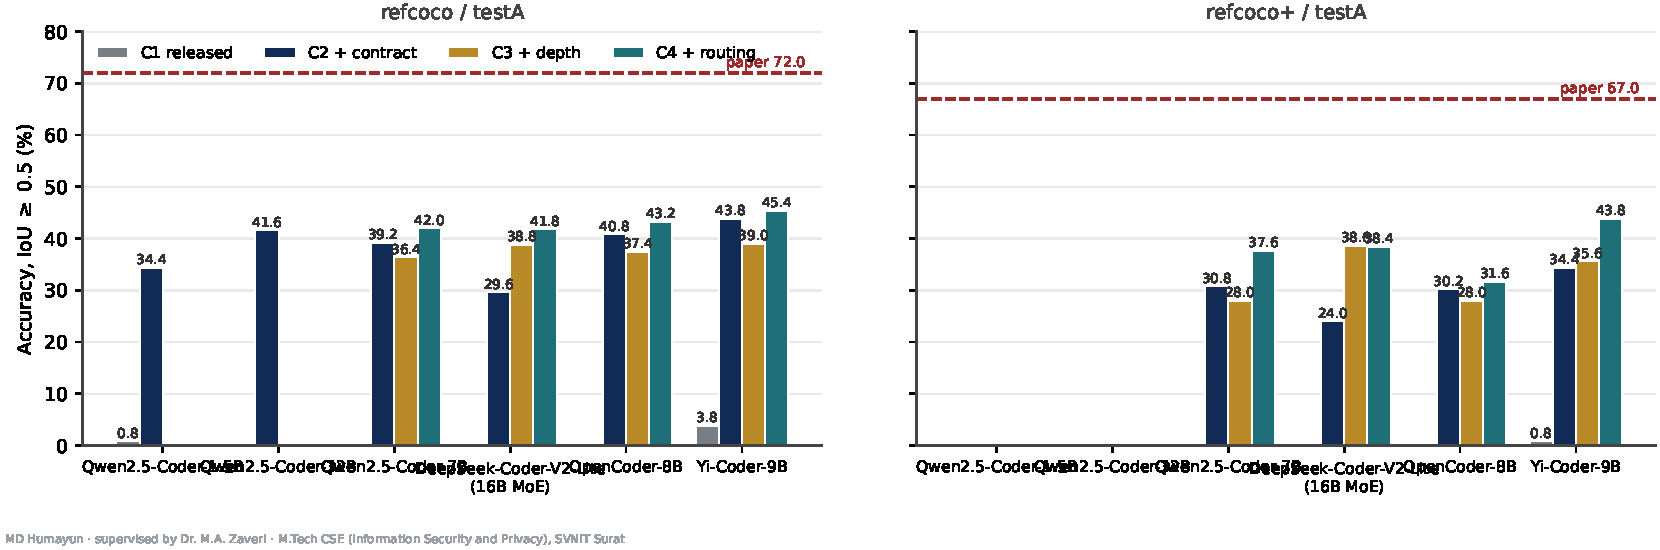
\includegraphics[width=\textwidth]{results/figures/fig17_grid.pdf}
\caption[Accuracy across all generators and conditions]{All four models under all
four conditions, both datasets. The dashed line is the paper's reported figure
($72.0$ on RefCOCO, $67.0$ on RefCOCO+). Every generator is near-zero under C1 and
recovers substantially by C2.}
\label{fig:m4-grid}
\end{figure}

\subsection{Q1 --- is the specification gap universal?}

\begin{table}[htbp]\centering
\caption{C1 $\to$ C2, RefCOCO overall. A gap present in every family cannot be a
property of one model.}
\label{tab:m4-q1}
\begin{tabular}{@{}lrrr@{}}
\toprule
\textbf{Generator} & \textbf{C1} & \textbf{C2} & \textbf{gain} \\
\midrule
Qwen2.5-Coder-1.5B & 0.80 & 34.40 & $+33.6$ \\
Qwen2.5-Coder-7B & 0.00 & 39.20 & $+39.2$ \\
Qwen2.5-Coder-32B & 0.00 & 41.60 & $+41.6$ \\
DeepSeek-V2-Lite & 0.00 & 29.60 & $+29.6$ \\
OpenCoder-8B & 0.20 & 40.80 & $+40.6$ \\
Yi-Coder-9B & 3.80 & 43.80 & $+40.0$ \\
\bottomrule
\end{tabular}
\end{table}

Every generator scores below $4\%$ under the released prompt, and every one recovers
by at least $29.6$ points under the return-type contract alone.
\textbf{The specification gap is not a Qwen-specific failure.} Yi-Coder's baseline of
$3.80$ is the least severe of the six, and it remains a near-total failure relative to
its own $43.80$ under C2.

\subsection{Q2 --- does the depth capability transfer?}

\begin{table}[htbp]\centering
\caption{C2 $\to$ C3 on the RefCOCO+ spatial subset ($n=47$; the depth-word queries).}
\label{tab:m4-q2}
\begin{tabular}{@{}lrrr@{}}
\toprule
\textbf{Generator} & \textbf{C2 spatial} & \textbf{C3 spatial} & \textbf{gain} \\
\midrule
Qwen2.5-Coder-7B & 4.26 & 19.15 & $+14.9$ \\
DeepSeek-V2-Lite & 14.89 & 27.66 & $+12.8$ \\
OpenCoder-8B & 23.40 & 17.02 & $-6.4$ \\
Yi-Coder-9B & 25.53 & 29.79 & $+4.3$ \\
\bottomrule
\end{tabular}
\end{table}

Three of four generators improve on the depth subset when the primitives are offered;
OpenCoder is the exception, losing $6.4$ points.

Two observations matter independently of that exception. First, \textbf{OpenCoder and
Yi-Coder already score far higher than Qwen under C2} --- $23.40$ and $25.53$ against
Qwen's $4.26$ --- \emph{before} any depth primitive is offered. Some generators are
evidently resolving depth relations by other means under the plain grounding contract,
a behaviour not investigated here. Second, Qwen shows both the lowest starting point
and the largest gain, consistent with it benefiting most from an explicit primitive
precisely because it had the least alternative strategy.

At $n=47$ a single query is worth $2.13$ percentage points, so these differences span
roughly two to seven samples. The ordering is informative; the magnitudes are not.

\subsection{Q3 --- is the routing rule necessary in every family?}

\begin{table}[htbp]\centering
\caption{C2 $\to$ C3 $\to$ C4 on the RefCOCO non-spatial subset --- the control
against which over-application of the depth primitives shows up.}
\label{tab:m4-q3}
\begin{tabular}{@{}lrrrrr@{}}
\toprule
\textbf{Generator} & \textbf{C2} & \textbf{C3} & \textbf{C4} & \textbf{C3 change} & \textbf{C4 change} \\
\midrule
Qwen2.5-Coder-7B & 45.97 & 36.02 & 48.82 & $-9.9$ & $+12.8$ \\
DeepSeek-V2-Lite & 31.28 & 45.50 & 50.71 & $+14.2$ & $+5.2$ \\
OpenCoder-8B & 47.87 & 36.49 & 45.97 & $-11.4$ & $+9.5$ \\
Yi-Coder-9B & 49.29 & 49.76 & 52.13 & $+0.5$ & $+2.4$ \\
\bottomrule
\end{tabular}
\end{table}

Two of four generators exhibit the over-application failure that motivated C4 in
Chapter~\ref{ch:results}: Qwen loses $9.9$ points of non-spatial accuracy under C3
and OpenCoder loses $11.4$, and both recover under C4. Yi-Coder does not exhibit it
--- its non-spatial accuracy is flat between C2 and C3 --- yet still gains $2.4$
points from the routing rule.

DeepSeek behaves differently again: its C2 non-spatial accuracy is anomalously low
($31.28$, against $45.97$--$49.29$ for the others), so C3 appears to \emph{gain}
$14.2$ points rather than lose them. This is better read as DeepSeek performing poorly
under C2 than as the depth primitives helping non-spatial queries. Its C2 figures are
the weakest in the grid on both datasets ($29.60$ and $24.00$ overall), which is
consistent with its $2.4$B active parameters.

\textbf{One exception to the C3 $\to$ C4 ordering.} On RefCOCO+, DeepSeek is the sole
generator for which C4 does not exceed C3 ($38.40$ against $38.60$, a $-0.2$
difference). Every other model, and DeepSeek itself on RefCOCO ($38.80 \to 41.80$),
shows $\text{C4} > \text{C3}$. A $0.2$-point difference is one sample in 500 and has
not been re-seeded; it is reported rather than smoothed over, and the claim that C4
improves on C3 is stated as holding in every generator on RefCOCO and in three of four
on RefCOCO+.

\subsection{Q4 --- does a stronger generator raise accuracy?}

\begin{table}[htbp]\centering
\caption{Best condition (C4) against the paper's reported figures.}
\label{tab:m4-q4}
\begin{tabular}{@{}lrrr@{}}
\toprule
\textbf{Generator} & \textbf{C4 RefCOCO} & \textbf{C4 RefCOCO+} & \textbf{share of 72.0 / 67.0} \\
\midrule
Qwen2.5-Coder-7B & 42.00 & 37.60 & 58\% / 56\% \\
DeepSeek-V2-Lite & 41.80 & 38.40 & 58\% / 57\% \\
OpenCoder-8B & 43.20 & 31.60 & 60\% / 47\% \\
Yi-Coder-9B & \textbf{45.40} & \textbf{43.80} & \textbf{63\% / 65\%} \\
\bottomrule
\end{tabular}
\end{table}

\begin{figure}[htbp]\centering
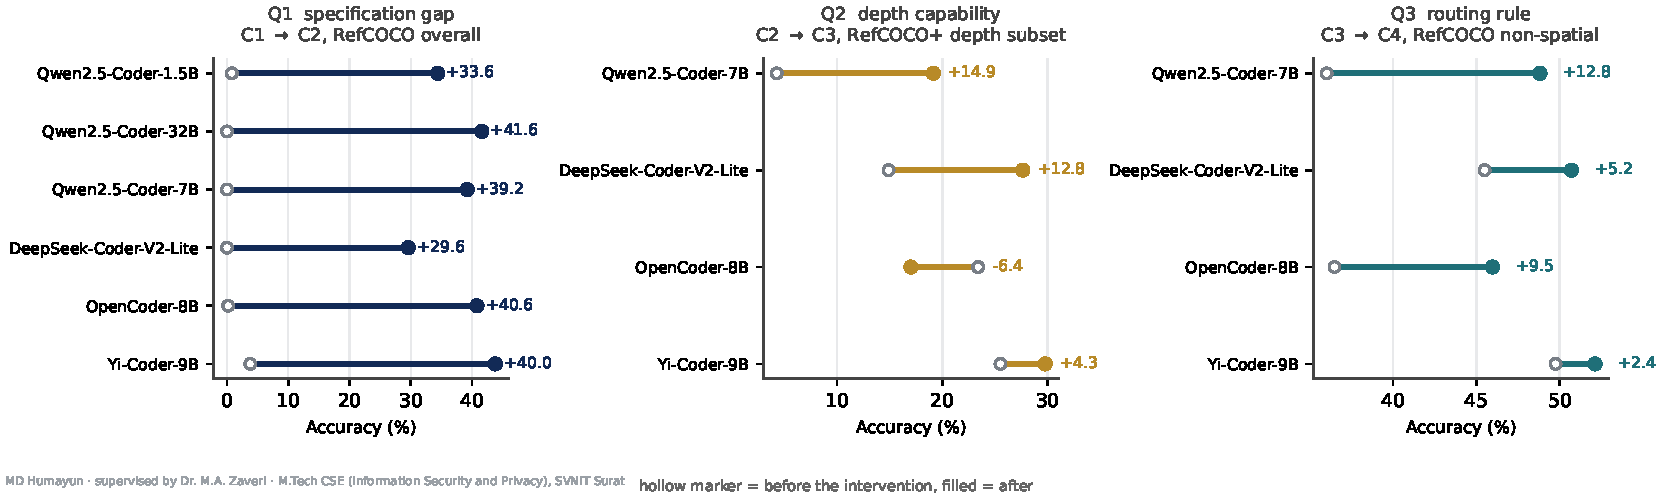
\includegraphics[width=\textwidth]{results/figures/fig18_generalisation.pdf}
\caption[Do the findings transfer across generators?]{Each panel answers one
generalisation question with a before-and-after marker per model: hollow before the
intervention, filled after. Left to right: the specification gap (Q1), the depth
capability (Q2), and the routing rule (Q3).}
\label{fig:m4-transfer}
\end{figure}

\textbf{Yi-Coder-9B is the strongest generator measured}, on both datasets, by $3.4$
points on RefCOCO and $6.2$ points on RefCOCO+ over Qwen2.5-Coder-7B. This answers
the question directly: \textbf{substituting a different open-weights generator does
raise accuracy, by three to six points, and does not close the gap to the paper's
reported figures.}

The perception ceiling measured independently of any generator ($81.5\%$ top-box
accuracy, held-out $n=200$) exceeds the paper's $72.0$, so the shortfall is not a
perception limit for any of the four generators tried. It remains a program-synthesis
limit --- which is measured support for treating the Codex substitution (D1) as the
dominant term in the gap rather than assuming it.

\section{Summary}

\begin{enumerate}[leftmargin=1.8em, itemsep=4pt]
\item The specification gap of Chapter~\ref{ch:results} is present in all six
generators measured, at severities from $0.00$ to $3.80$ under C1, and is repaired to
between $29.6$ and $43.8$ under C2. It is a property of the prompt, not of one vendor.

\item The depth capability transfers in three of four families. OpenCoder is an
exception on the depth subset. Two generators show substantially better depth
performance than Qwen even under the plain grounding contract, indicating a
generator-dependent alternative strategy not investigated here.

\item The over-application failure that motivated the routing rule is present in two
of four families and absent in the other two, yet C4 improves on C3 for every
generator on RefCOCO and for three of four on RefCOCO+. The routing rule helps whether
or not the specific failure it was designed to prevent is present.

\item Substituting the generator raises accuracy by three to six points at best
(Yi-Coder-9B) and does not close the gap to the paper. The gap is attributable to
program synthesis rather than to perception.
\end{enumerate}

\section{Limitations specific to this milestone}

\begin{enumerate}[leftmargin=1.6em, itemsep=3pt]
\item DeepSeek-Coder-V2-Lite's active parameter count ($2.4$B) is not comparable to
the three dense models ($7$--$9$B); its results are confounded by architecture and
capacity simultaneously. Its consistently weak C2 figures are the clearest symptom.

\item All four generators postdate Codex by two to three years. The grid tests family
and instruction-tuning lineage at a roughly fixed point in time, not model era.

\item Qwen2.5-Coder-1.5B and -32B were not extended to the full grid; only the 7B
point is shared between the scale sweep and the family sweep. The two answer different
questions and were run to answer each independently (D18).

\item Every cell is single-seed and greedy. The DeepSeek C3/C4 near-tie on RefCOCO+
in particular has not been re-seeded and should be treated as inconclusive rather than
as a genuine reversal.

\item The RefCOCO+ depth subset is $n=47$, so each query is worth $2.13$ percentage
points. Several models land on identical values there ($19.15\% = 9/47$), which is a
consequence of the quantisation rather than a meaningful agreement.
\end{enumerate}

% =====================================================================
\chapter{Milestone 4 --- Generalisation Across Generator Families}
\label{ch:milestone4}

\section{Motivation}

Every result in Chapters~\ref{ch:results} and~\ref{ch:rejected} is measured on one
generator family: Qwen2.5-Coder, at 1.5B, 7B and 32B parameters. The scale sweep
shows that the specification gap and the flat spatial accuracy persist across that
range, which rules out capacity \emph{within} the Qwen family as an explanation. It
does not rule out the family itself. A reader can reasonably ask whether the released
prompt's failure is a property of ViperGPT's specification or a property of how one
vendor's models happen to follow instructions --- and, separately, whether a stronger
publicly available generator narrows the gap to the paper's reported $72.0$.

This chapter answers both with a second, orthogonal sweep: four model families across
all four prompt conditions on both datasets.

\section{Design}

\begin{table}[htbp]\centering\small
\caption{The four generators. All are openly downloadable without licence acceptance
or an access token, so the grid is reproducible without credential management --- a
deliberate choice, given that the dissertation's subject is a system rendered
irreproducible by a withdrawn proprietary model.}
\label{tab:m4-models}
\begin{tabular}{@{}llll@{}}
\toprule
\textbf{Generator} & \textbf{Publisher} & \textbf{Parameters} & \textbf{Note} \\
\midrule
Qwen2.5-Coder-7B-Instruct & Alibaba & 7B dense & used throughout Ch.~\ref{ch:results} \\
DeepSeek-Coder-V2-Lite-Instruct & DeepSeek & 16B / \textbf{2.4B active} & mixture-of-experts \\
Yi-Coder-9B-Chat & 01.AI & 9B dense & --- \\
OpenCoder-8B-Instruct & INF / M-A-P & 8B dense & needs \texttt{trust\_remote\_code} (D15) \\
\bottomrule
\end{tabular}
\end{table}

Each model was run under all four prompt conditions (C1--C4,
Section~\ref{sec:prompts}) on both datasets at $n=500$ with greedy decoding --- the
same protocol as every other result in this dissertation. Combined with the existing
Qwen-7B cells this gives a $4 \times 4 \times 2 = 32$-cell grid. Qwen2.5-Coder-1.5B
and -32B contribute C1 and C2 on RefCOCO from the earlier scale sweep and are
included in the C1$\to$C2 analysis only (D18).

\textbf{What the design isolates.} The prompt conditions are unchanged; only the
generator varies. A difference between models under the same condition is therefore
attributable to the generator, and a difference between conditions that holds across
all four generators is attributable to the prompt rather than to one vendor's
instruction-following.

\textbf{What it does not control for.} DeepSeek-Coder-V2-Lite is a mixture-of-experts
model with 16B total parameters but only 2.4B active per token --- roughly a third of
the smallest dense model here. Any DeepSeek result is confounded by architecture and
effective capacity simultaneously and is reported as such rather than treated as
size-matched. All four generators were released in 2024--2025, two to three years
after Codex, so the grid is not a controlled test of model era.

\section{Engineering}

Three failures occurred while building the grid. Two are general lessons rather than
incidental bugs.

\subsection{A global flag broke the model it was not meant for}

OpenCoder ships custom tokenizer and model classes and requires
\texttt{trust\_remote\_code=True}. Setting the flag globally broke DeepSeek: it forced
\texttt{transformers} to load the repository's own \texttt{modeling\_deepseek.py} in
preference to the library's built-in class, and that file imports
\texttt{is\_torch\_fx\_available}, removed in \texttt{transformers}~5.x.

\begin{lstlisting}[caption={The flag is made conditional on the model identifier
rather than applied uniformly (D15).}]
tok = AutoTokenizer.from_pretrained(
    a.model, padding_side="left",
    trust_remote_code=("OpenCoder" in a.model))
\end{lstlisting}

\subsection{A resumability bug reported failure as success}

The generation script creates its run directory \emph{before} loading the model, so
when the flag above crashed DeepSeek at model-load time, eight empty directories were
left behind. The grid driver's resume logic checked only for the directory's
existence, so the next submission treated all eight as complete, skipped them, and
reported success having generated nothing.

\begin{lstlisting}[caption={Completion is tested by the artefact, not by the
container created to hold it.}]
EXPECT="outputs/runs/*m1_${DS}_testA_${SHORT}_${TAG}_greedy"
if compgen -G "$EXPECT/programs.jsonl" > /dev/null; then
    echo ">>> SKIP  $DS | $PROMPT  (already generated)"
    continue
fi
\end{lstlisting}

This generalises beyond the project: in a resumable pipeline the marker of completion
must be the output artefact, never a side effect of having started.

\subsection{A batching corruption, not a crash}

After both fixes, DeepSeek's RefCOCO/C1 cell generated at batch size 6 --- the setting
used for the other models --- with a parse rate of $0.4\%$ across 500 samples. Not an
error; near-total corruption. Regenerating at batch size 1 (D17) restored the parse
rate to the range seen on the model's other seven cells. The root cause was not fully
diagnosed since a working fix was found, and it is recorded as a fragility of this
particular mixture-of-experts model under batched greedy decoding on this stack rather
than assumed to generalise.

\section{Results}

\begin{table}[htbp]\centering\small
\caption{Accuracy at IoU $\geq 0.5$, greedy, $n=500$ per cell, testA. Conditions as
defined in Table~\ref{tab:conditions}.}
\label{tab:m4-main}
\begin{tabular}{@{}lrrrrrrrr@{}}
\toprule
& \multicolumn{4}{c}{\textbf{RefCOCO}} & \multicolumn{4}{c}{\textbf{RefCOCO+}} \\
\cmidrule(lr){2-5}\cmidrule(lr){6-9}
\textbf{Generator} & C1 & C2 & C3 & C4 & C1 & C2 & C3 & C4 \\
\midrule
Qwen2.5-Coder-7B & 0.00 & 39.20 & 36.40 & 42.00 & 0.00 & 30.80 & 28.00 & 37.60 \\
DeepSeek-V2-Lite & 0.00 & 29.60 & 38.80 & 41.80 & 0.00 & 24.00 & 38.60 & 38.40 \\
OpenCoder-8B & 0.20 & 40.80 & 37.40 & 43.20 & 0.00 & 30.20 & 28.00 & 31.60 \\
Yi-Coder-9B & 3.80 & 43.80 & 39.00 & \textbf{45.40} & 0.80 & 34.40 & 35.60 & \textbf{43.80} \\
\bottomrule
\end{tabular}
\end{table}

\begin{figure}[htbp]\centering
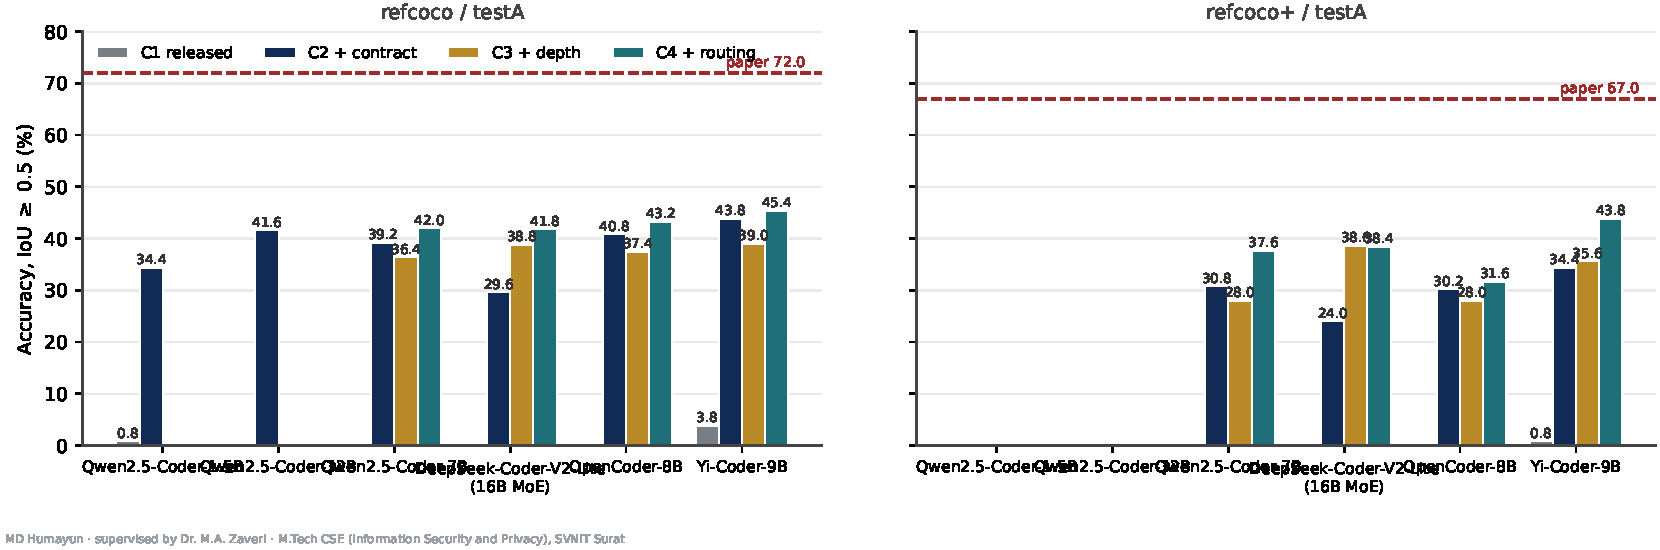
\includegraphics[width=\textwidth]{results/figures/fig17_grid.pdf}
\caption[Accuracy across all generators and conditions]{All four models under all
four conditions, both datasets. The dashed line is the paper's reported figure
($72.0$ on RefCOCO, $67.0$ on RefCOCO+). Every generator is near-zero under C1 and
recovers substantially by C2.}
\label{fig:m4-grid}
\end{figure}

\subsection{Q1 --- is the specification gap universal?}

\begin{table}[htbp]\centering
\caption{C1 $\to$ C2, RefCOCO overall. A gap present in every family cannot be a
property of one model.}
\label{tab:m4-q1}
\begin{tabular}{@{}lrrr@{}}
\toprule
\textbf{Generator} & \textbf{C1} & \textbf{C2} & \textbf{gain} \\
\midrule
Qwen2.5-Coder-1.5B & 0.80 & 34.40 & $+33.6$ \\
Qwen2.5-Coder-7B & 0.00 & 39.20 & $+39.2$ \\
Qwen2.5-Coder-32B & 0.00 & 41.60 & $+41.6$ \\
DeepSeek-V2-Lite & 0.00 & 29.60 & $+29.6$ \\
OpenCoder-8B & 0.20 & 40.80 & $+40.6$ \\
Yi-Coder-9B & 3.80 & 43.80 & $+40.0$ \\
\bottomrule
\end{tabular}
\end{table}

Every generator scores below $4\%$ under the released prompt, and every one recovers
by at least $29.6$ points under the return-type contract alone.
\textbf{The specification gap is not a Qwen-specific failure.} Yi-Coder's baseline of
$3.80$ is the least severe of the six, and it remains a near-total failure relative to
its own $43.80$ under C2.

\subsection{Q2 --- does the depth capability transfer?}

\begin{table}[htbp]\centering
\caption{C2 $\to$ C3 on the RefCOCO+ spatial subset ($n=47$; the depth-word queries).}
\label{tab:m4-q2}
\begin{tabular}{@{}lrrr@{}}
\toprule
\textbf{Generator} & \textbf{C2 spatial} & \textbf{C3 spatial} & \textbf{gain} \\
\midrule
Qwen2.5-Coder-7B & 4.26 & 19.15 & $+14.9$ \\
DeepSeek-V2-Lite & 14.89 & 27.66 & $+12.8$ \\
OpenCoder-8B & 23.40 & 17.02 & $-6.4$ \\
Yi-Coder-9B & 25.53 & 29.79 & $+4.3$ \\
\bottomrule
\end{tabular}
\end{table}

Three of four generators improve on the depth subset when the primitives are offered;
OpenCoder is the exception, losing $6.4$ points.

Two observations matter independently of that exception. First, \textbf{OpenCoder and
Yi-Coder already score far higher than Qwen under C2} --- $23.40$ and $25.53$ against
Qwen's $4.26$ --- \emph{before} any depth primitive is offered. Some generators are
evidently resolving depth relations by other means under the plain grounding contract,
a behaviour not investigated here. Second, Qwen shows both the lowest starting point
and the largest gain, consistent with it benefiting most from an explicit primitive
precisely because it had the least alternative strategy.

At $n=47$ a single query is worth $2.13$ percentage points, so these differences span
roughly two to seven samples. The ordering is informative; the magnitudes are not.

\subsection{Q3 --- is the routing rule necessary in every family?}

\begin{table}[htbp]\centering
\caption{C2 $\to$ C3 $\to$ C4 on the RefCOCO non-spatial subset --- the control
against which over-application of the depth primitives shows up.}
\label{tab:m4-q3}
\begin{tabular}{@{}lrrrrr@{}}
\toprule
\textbf{Generator} & \textbf{C2} & \textbf{C3} & \textbf{C4} & \textbf{C3 change} & \textbf{C4 change} \\
\midrule
Qwen2.5-Coder-7B & 45.97 & 36.02 & 48.82 & $-9.9$ & $+12.8$ \\
DeepSeek-V2-Lite & 31.28 & 45.50 & 50.71 & $+14.2$ & $+5.2$ \\
OpenCoder-8B & 47.87 & 36.49 & 45.97 & $-11.4$ & $+9.5$ \\
Yi-Coder-9B & 49.29 & 49.76 & 52.13 & $+0.5$ & $+2.4$ \\
\bottomrule
\end{tabular}
\end{table}

Two of four generators exhibit the over-application failure that motivated C4 in
Chapter~\ref{ch:results}: Qwen loses $9.9$ points of non-spatial accuracy under C3
and OpenCoder loses $11.4$, and both recover under C4. Yi-Coder does not exhibit it
--- its non-spatial accuracy is flat between C2 and C3 --- yet still gains $2.4$
points from the routing rule.

DeepSeek behaves differently again: its C2 non-spatial accuracy is anomalously low
($31.28$, against $45.97$--$49.29$ for the others), so C3 appears to \emph{gain}
$14.2$ points rather than lose them. This is better read as DeepSeek performing poorly
under C2 than as the depth primitives helping non-spatial queries. Its C2 figures are
the weakest in the grid on both datasets ($29.60$ and $24.00$ overall), which is
consistent with its $2.4$B active parameters.

\textbf{One exception to the C3 $\to$ C4 ordering.} On RefCOCO+, DeepSeek is the sole
generator for which C4 does not exceed C3 ($38.40$ against $38.60$, a $-0.2$
difference). Every other model, and DeepSeek itself on RefCOCO ($38.80 \to 41.80$),
shows $\text{C4} > \text{C3}$. A $0.2$-point difference is one sample in 500 and has
not been re-seeded; it is reported rather than smoothed over, and the claim that C4
improves on C3 is stated as holding in every generator on RefCOCO and in three of four
on RefCOCO+.

\subsection{Q4 --- does a stronger generator raise accuracy?}

\begin{table}[htbp]\centering
\caption{Best condition (C4) against the paper's reported figures.}
\label{tab:m4-q4}
\begin{tabular}{@{}lrrr@{}}
\toprule
\textbf{Generator} & \textbf{C4 RefCOCO} & \textbf{C4 RefCOCO+} & \textbf{share of 72.0 / 67.0} \\
\midrule
Qwen2.5-Coder-7B & 42.00 & 37.60 & 58\% / 56\% \\
DeepSeek-V2-Lite & 41.80 & 38.40 & 58\% / 57\% \\
OpenCoder-8B & 43.20 & 31.60 & 60\% / 47\% \\
Yi-Coder-9B & \textbf{45.40} & \textbf{43.80} & \textbf{63\% / 65\%} \\
\bottomrule
\end{tabular}
\end{table}

\begin{figure}[htbp]\centering
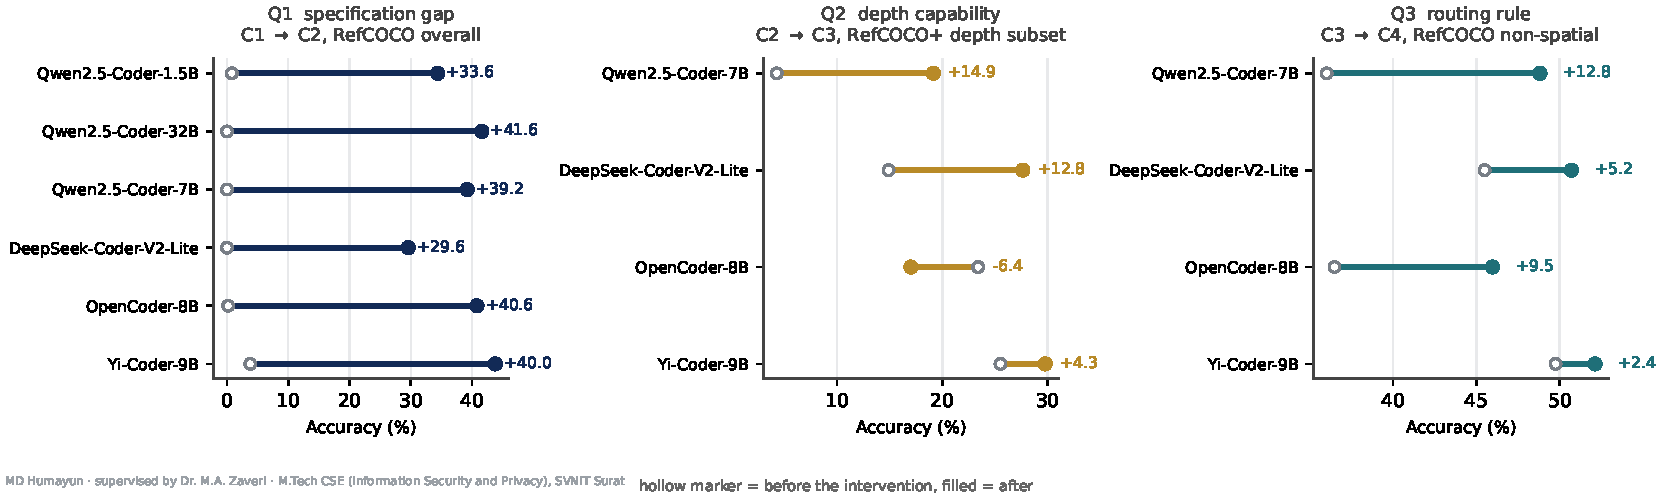
\includegraphics[width=\textwidth]{results/figures/fig18_generalisation.pdf}
\caption[Do the findings transfer across generators?]{Each panel answers one
generalisation question with a before-and-after marker per model: hollow before the
intervention, filled after. Left to right: the specification gap (Q1), the depth
capability (Q2), and the routing rule (Q3).}
\label{fig:m4-transfer}
\end{figure}

\textbf{Yi-Coder-9B is the strongest generator measured}, on both datasets, by $3.4$
points on RefCOCO and $6.2$ points on RefCOCO+ over Qwen2.5-Coder-7B. This answers
the question directly: \textbf{substituting a different open-weights generator does
raise accuracy, by three to six points, and does not close the gap to the paper's
reported figures.}

The perception ceiling measured independently of any generator ($81.5\%$ top-box
accuracy, held-out $n=200$) exceeds the paper's $72.0$, so the shortfall is not a
perception limit for any of the four generators tried. It remains a program-synthesis
limit --- which is measured support for treating the Codex substitution (D1) as the
dominant term in the gap rather than assuming it.

\section{Summary}

\begin{enumerate}[leftmargin=1.8em, itemsep=4pt]
\item The specification gap of Chapter~\ref{ch:results} is present in all six
generators measured, at severities from $0.00$ to $3.80$ under C1, and is repaired to
between $29.6$ and $43.8$ under C2. It is a property of the prompt, not of one vendor.

\item The depth capability transfers in three of four families. OpenCoder is an
exception on the depth subset. Two generators show substantially better depth
performance than Qwen even under the plain grounding contract, indicating a
generator-dependent alternative strategy not investigated here.

\item The over-application failure that motivated the routing rule is present in two
of four families and absent in the other two, yet C4 improves on C3 for every
generator on RefCOCO and for three of four on RefCOCO+. The routing rule helps whether
or not the specific failure it was designed to prevent is present.

\item Substituting the generator raises accuracy by three to six points at best
(Yi-Coder-9B) and does not close the gap to the paper. The gap is attributable to
program synthesis rather than to perception.
\end{enumerate}

\section{Limitations specific to this milestone}

\begin{enumerate}[leftmargin=1.6em, itemsep=3pt]
\item DeepSeek-Coder-V2-Lite's active parameter count ($2.4$B) is not comparable to
the three dense models ($7$--$9$B); its results are confounded by architecture and
capacity simultaneously. Its consistently weak C2 figures are the clearest symptom.

\item All four generators postdate Codex by two to three years. The grid tests family
and instruction-tuning lineage at a roughly fixed point in time, not model era.

\item Qwen2.5-Coder-1.5B and -32B were not extended to the full grid; only the 7B
point is shared between the scale sweep and the family sweep. The two answer different
questions and were run to answer each independently (D18).

\item Every cell is single-seed and greedy. The DeepSeek C3/C4 near-tie on RefCOCO+
in particular has not been re-seeded and should be treated as inconclusive rather than
as a genuine reversal.

\item The RefCOCO+ depth subset is $n=47$, so each query is worth $2.13$ percentage
points. Several models land on identical values there ($19.15\% = 9/47$), which is a
consequence of the quantisation rather than a meaningful agreement.
\end{enumerate}

% =====================================================================
\chapter{Milestone 4 --- Generalisation Across Generator Families}
\label{ch:milestone4}

\section{Motivation}

Every result in Chapters~\ref{ch:results} and~\ref{ch:rejected} is measured on one
generator family: Qwen2.5-Coder, at 1.5B, 7B and 32B parameters. The scale sweep
shows that the specification gap and the flat spatial accuracy persist across that
range, which rules out capacity \emph{within} the Qwen family as an explanation. It
does not rule out the family itself. A reader can reasonably ask whether the released
prompt's failure is a property of ViperGPT's specification or a property of how one
vendor's models happen to follow instructions --- and, separately, whether a stronger
publicly available generator narrows the gap to the paper's reported $72.0$.

This chapter answers both with a second, orthogonal sweep: four model families across
all four prompt conditions on both datasets.

\section{Design}

\begin{table}[htbp]\centering\small
\caption{The four generators. All are openly downloadable without licence acceptance
or an access token, so the grid is reproducible without credential management --- a
deliberate choice, given that the dissertation's subject is a system rendered
irreproducible by a withdrawn proprietary model.}
\label{tab:m4-models}
\begin{tabular}{@{}llll@{}}
\toprule
\textbf{Generator} & \textbf{Publisher} & \textbf{Parameters} & \textbf{Note} \\
\midrule
Qwen2.5-Coder-7B-Instruct & Alibaba & 7B dense & used throughout Ch.~\ref{ch:results} \\
DeepSeek-Coder-V2-Lite-Instruct & DeepSeek & 16B / \textbf{2.4B active} & mixture-of-experts \\
Yi-Coder-9B-Chat & 01.AI & 9B dense & --- \\
OpenCoder-8B-Instruct & INF / M-A-P & 8B dense & needs \texttt{trust\_remote\_code} (D15) \\
\bottomrule
\end{tabular}
\end{table}

Each model was run under all four prompt conditions (C1--C4,
Section~\ref{sec:prompts}) on both datasets at $n=500$ with greedy decoding --- the
same protocol as every other result in this dissertation. Combined with the existing
Qwen-7B cells this gives a $4 \times 4 \times 2 = 32$-cell grid. Qwen2.5-Coder-1.5B
and -32B contribute C1 and C2 on RefCOCO from the earlier scale sweep and are
included in the C1$\to$C2 analysis only (D18).

\textbf{What the design isolates.} The prompt conditions are unchanged; only the
generator varies. A difference between models under the same condition is therefore
attributable to the generator, and a difference between conditions that holds across
all four generators is attributable to the prompt rather than to one vendor's
instruction-following.

\textbf{What it does not control for.} DeepSeek-Coder-V2-Lite is a mixture-of-experts
model with 16B total parameters but only 2.4B active per token --- roughly a third of
the smallest dense model here. Any DeepSeek result is confounded by architecture and
effective capacity simultaneously and is reported as such rather than treated as
size-matched. All four generators were released in 2024--2025, two to three years
after Codex, so the grid is not a controlled test of model era.

\section{Engineering}

Three failures occurred while building the grid. Two are general lessons rather than
incidental bugs.

\subsection{A global flag broke the model it was not meant for}

OpenCoder ships custom tokenizer and model classes and requires
\texttt{trust\_remote\_code=True}. Setting the flag globally broke DeepSeek: it forced
\texttt{transformers} to load the repository's own \texttt{modeling\_deepseek.py} in
preference to the library's built-in class, and that file imports
\texttt{is\_torch\_fx\_available}, removed in \texttt{transformers}~5.x.

\begin{lstlisting}[caption={The flag is made conditional on the model identifier
rather than applied uniformly (D15).}]
tok = AutoTokenizer.from_pretrained(
    a.model, padding_side="left",
    trust_remote_code=("OpenCoder" in a.model))
\end{lstlisting}

\subsection{A resumability bug reported failure as success}

The generation script creates its run directory \emph{before} loading the model, so
when the flag above crashed DeepSeek at model-load time, eight empty directories were
left behind. The grid driver's resume logic checked only for the directory's
existence, so the next submission treated all eight as complete, skipped them, and
reported success having generated nothing.

\begin{lstlisting}[caption={Completion is tested by the artefact, not by the
container created to hold it.}]
EXPECT="outputs/runs/*m1_${DS}_testA_${SHORT}_${TAG}_greedy"
if compgen -G "$EXPECT/programs.jsonl" > /dev/null; then
    echo ">>> SKIP  $DS | $PROMPT  (already generated)"
    continue
fi
\end{lstlisting}

This generalises beyond the project: in a resumable pipeline the marker of completion
must be the output artefact, never a side effect of having started.

\subsection{A batching corruption, not a crash}

After both fixes, DeepSeek's RefCOCO/C1 cell generated at batch size 6 --- the setting
used for the other models --- with a parse rate of $0.4\%$ across 500 samples. Not an
error; near-total corruption. Regenerating at batch size 1 (D17) restored the parse
rate to the range seen on the model's other seven cells. The root cause was not fully
diagnosed since a working fix was found, and it is recorded as a fragility of this
particular mixture-of-experts model under batched greedy decoding on this stack rather
than assumed to generalise.

\section{Results}

\begin{table}[htbp]\centering\small
\caption{Accuracy at IoU $\geq 0.5$, greedy, $n=500$ per cell, testA. Conditions as
defined in Table~\ref{tab:conditions}.}
\label{tab:m4-main}
\begin{tabular}{@{}lrrrrrrrr@{}}
\toprule
& \multicolumn{4}{c}{\textbf{RefCOCO}} & \multicolumn{4}{c}{\textbf{RefCOCO+}} \\
\cmidrule(lr){2-5}\cmidrule(lr){6-9}
\textbf{Generator} & C1 & C2 & C3 & C4 & C1 & C2 & C3 & C4 \\
\midrule
Qwen2.5-Coder-7B & 0.00 & 39.20 & 36.40 & 42.00 & 0.00 & 30.80 & 28.00 & 37.60 \\
DeepSeek-V2-Lite & 0.00 & 29.60 & 38.80 & 41.80 & 0.00 & 24.00 & 38.60 & 38.40 \\
OpenCoder-8B & 0.20 & 40.80 & 37.40 & 43.20 & 0.00 & 30.20 & 28.00 & 31.60 \\
Yi-Coder-9B & 3.80 & 43.80 & 39.00 & \textbf{45.40} & 0.80 & 34.40 & 35.60 & \textbf{43.80} \\
\bottomrule
\end{tabular}
\end{table}

\begin{figure}[htbp]\centering
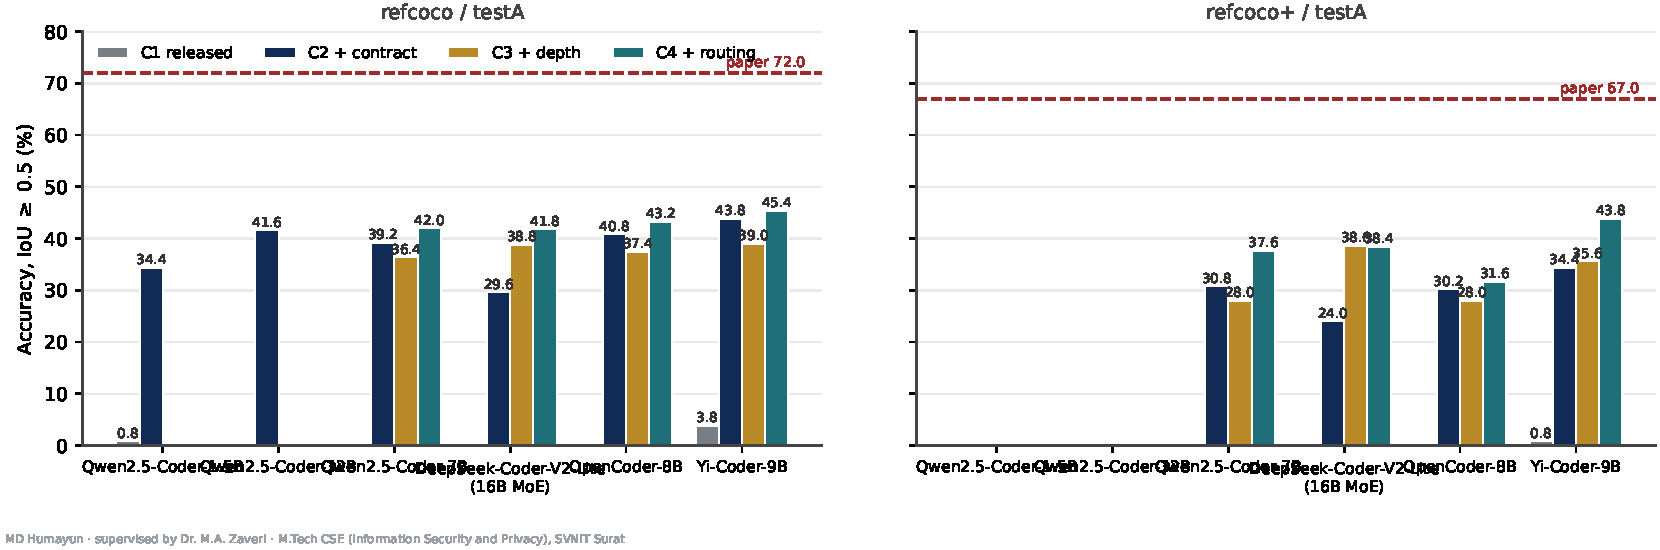
\includegraphics[width=\textwidth]{results/figures/fig17_grid.pdf}
\caption[Accuracy across all generators and conditions]{All four models under all
four conditions, both datasets. The dashed line is the paper's reported figure
($72.0$ on RefCOCO, $67.0$ on RefCOCO+). Every generator is near-zero under C1 and
recovers substantially by C2.}
\label{fig:m4-grid}
\end{figure}

\subsection{Q1 --- is the specification gap universal?}

\begin{table}[htbp]\centering
\caption{C1 $\to$ C2, RefCOCO overall. A gap present in every family cannot be a
property of one model.}
\label{tab:m4-q1}
\begin{tabular}{@{}lrrr@{}}
\toprule
\textbf{Generator} & \textbf{C1} & \textbf{C2} & \textbf{gain} \\
\midrule
Qwen2.5-Coder-1.5B & 0.80 & 34.40 & $+33.6$ \\
Qwen2.5-Coder-7B & 0.00 & 39.20 & $+39.2$ \\
Qwen2.5-Coder-32B & 0.00 & 41.60 & $+41.6$ \\
DeepSeek-V2-Lite & 0.00 & 29.60 & $+29.6$ \\
OpenCoder-8B & 0.20 & 40.80 & $+40.6$ \\
Yi-Coder-9B & 3.80 & 43.80 & $+40.0$ \\
\bottomrule
\end{tabular}
\end{table}

Every generator scores below $4\%$ under the released prompt, and every one recovers
by at least $29.6$ points under the return-type contract alone.
\textbf{The specification gap is not a Qwen-specific failure.} Yi-Coder's baseline of
$3.80$ is the least severe of the six, and it remains a near-total failure relative to
its own $43.80$ under C2.

\subsection{Q2 --- does the depth capability transfer?}

\begin{table}[htbp]\centering
\caption{C2 $\to$ C3 on the RefCOCO+ spatial subset ($n=47$; the depth-word queries).}
\label{tab:m4-q2}
\begin{tabular}{@{}lrrr@{}}
\toprule
\textbf{Generator} & \textbf{C2 spatial} & \textbf{C3 spatial} & \textbf{gain} \\
\midrule
Qwen2.5-Coder-7B & 4.26 & 19.15 & $+14.9$ \\
DeepSeek-V2-Lite & 14.89 & 27.66 & $+12.8$ \\
OpenCoder-8B & 23.40 & 17.02 & $-6.4$ \\
Yi-Coder-9B & 25.53 & 29.79 & $+4.3$ \\
\bottomrule
\end{tabular}
\end{table}

Three of four generators improve on the depth subset when the primitives are offered;
OpenCoder is the exception, losing $6.4$ points.

Two observations matter independently of that exception. First, \textbf{OpenCoder and
Yi-Coder already score far higher than Qwen under C2} --- $23.40$ and $25.53$ against
Qwen's $4.26$ --- \emph{before} any depth primitive is offered. Some generators are
evidently resolving depth relations by other means under the plain grounding contract,
a behaviour not investigated here. Second, Qwen shows both the lowest starting point
and the largest gain, consistent with it benefiting most from an explicit primitive
precisely because it had the least alternative strategy.

At $n=47$ a single query is worth $2.13$ percentage points, so these differences span
roughly two to seven samples. The ordering is informative; the magnitudes are not.

\subsection{Q3 --- is the routing rule necessary in every family?}

\begin{table}[htbp]\centering
\caption{C2 $\to$ C3 $\to$ C4 on the RefCOCO non-spatial subset --- the control
against which over-application of the depth primitives shows up.}
\label{tab:m4-q3}
\begin{tabular}{@{}lrrrrr@{}}
\toprule
\textbf{Generator} & \textbf{C2} & \textbf{C3} & \textbf{C4} & \textbf{C3 change} & \textbf{C4 change} \\
\midrule
Qwen2.5-Coder-7B & 45.97 & 36.02 & 48.82 & $-9.9$ & $+12.8$ \\
DeepSeek-V2-Lite & 31.28 & 45.50 & 50.71 & $+14.2$ & $+5.2$ \\
OpenCoder-8B & 47.87 & 36.49 & 45.97 & $-11.4$ & $+9.5$ \\
Yi-Coder-9B & 49.29 & 49.76 & 52.13 & $+0.5$ & $+2.4$ \\
\bottomrule
\end{tabular}
\end{table}

Two of four generators exhibit the over-application failure that motivated C4 in
Chapter~\ref{ch:results}: Qwen loses $9.9$ points of non-spatial accuracy under C3
and OpenCoder loses $11.4$, and both recover under C4. Yi-Coder does not exhibit it
--- its non-spatial accuracy is flat between C2 and C3 --- yet still gains $2.4$
points from the routing rule.

DeepSeek behaves differently again: its C2 non-spatial accuracy is anomalously low
($31.28$, against $45.97$--$49.29$ for the others), so C3 appears to \emph{gain}
$14.2$ points rather than lose them. This is better read as DeepSeek performing poorly
under C2 than as the depth primitives helping non-spatial queries. Its C2 figures are
the weakest in the grid on both datasets ($29.60$ and $24.00$ overall), which is
consistent with its $2.4$B active parameters.

\textbf{One exception to the C3 $\to$ C4 ordering.} On RefCOCO+, DeepSeek is the sole
generator for which C4 does not exceed C3 ($38.40$ against $38.60$, a $-0.2$
difference). Every other model, and DeepSeek itself on RefCOCO ($38.80 \to 41.80$),
shows $\text{C4} > \text{C3}$. A $0.2$-point difference is one sample in 500 and has
not been re-seeded; it is reported rather than smoothed over, and the claim that C4
improves on C3 is stated as holding in every generator on RefCOCO and in three of four
on RefCOCO+.

\subsection{Q4 --- does a stronger generator raise accuracy?}

\begin{table}[htbp]\centering
\caption{Best condition (C4) against the paper's reported figures.}
\label{tab:m4-q4}
\begin{tabular}{@{}lrrr@{}}
\toprule
\textbf{Generator} & \textbf{C4 RefCOCO} & \textbf{C4 RefCOCO+} & \textbf{share of 72.0 / 67.0} \\
\midrule
Qwen2.5-Coder-7B & 42.00 & 37.60 & 58\% / 56\% \\
DeepSeek-V2-Lite & 41.80 & 38.40 & 58\% / 57\% \\
OpenCoder-8B & 43.20 & 31.60 & 60\% / 47\% \\
Yi-Coder-9B & \textbf{45.40} & \textbf{43.80} & \textbf{63\% / 65\%} \\
\bottomrule
\end{tabular}
\end{table}

\begin{figure}[htbp]\centering
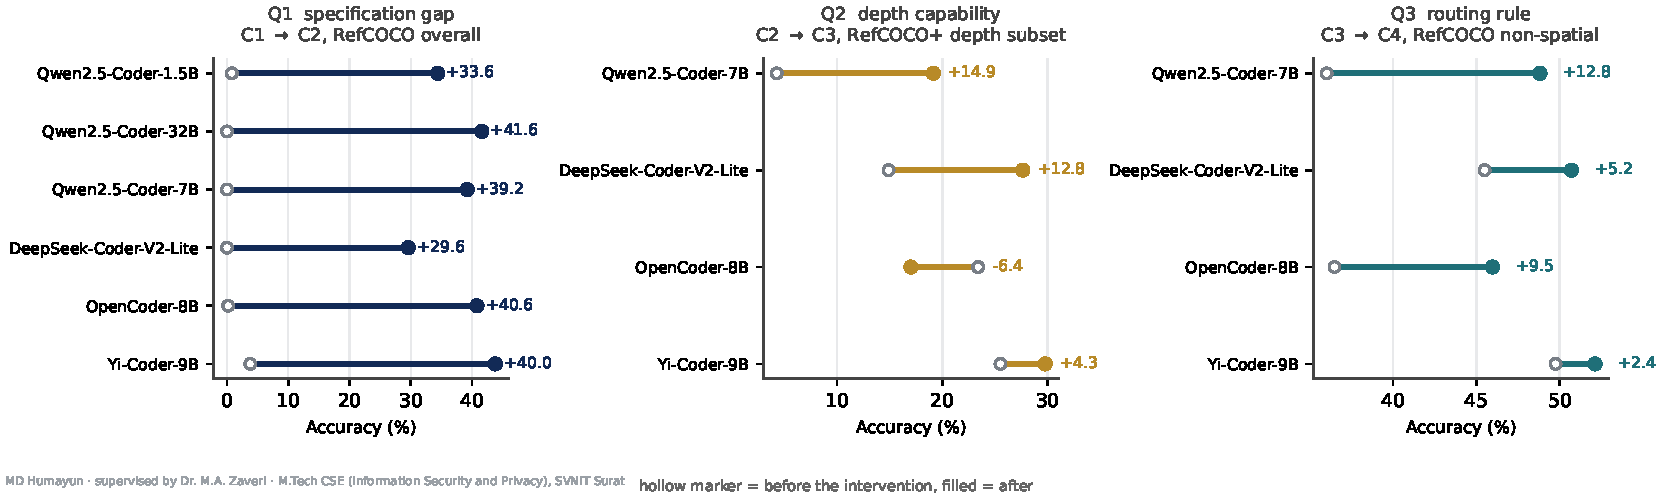
\includegraphics[width=\textwidth]{results/figures/fig18_generalisation.pdf}
\caption[Do the findings transfer across generators?]{Each panel answers one
generalisation question with a before-and-after marker per model: hollow before the
intervention, filled after. Left to right: the specification gap (Q1), the depth
capability (Q2), and the routing rule (Q3).}
\label{fig:m4-transfer}
\end{figure}

\textbf{Yi-Coder-9B is the strongest generator measured}, on both datasets, by $3.4$
points on RefCOCO and $6.2$ points on RefCOCO+ over Qwen2.5-Coder-7B. This answers
the question directly: \textbf{substituting a different open-weights generator does
raise accuracy, by three to six points, and does not close the gap to the paper's
reported figures.}

The perception ceiling measured independently of any generator ($81.5\%$ top-box
accuracy, held-out $n=200$) exceeds the paper's $72.0$, so the shortfall is not a
perception limit for any of the four generators tried. It remains a program-synthesis
limit --- which is measured support for treating the Codex substitution (D1) as the
dominant term in the gap rather than assuming it.

\section{Summary}

\begin{enumerate}[leftmargin=1.8em, itemsep=4pt]
\item The specification gap of Chapter~\ref{ch:results} is present in all six
generators measured, at severities from $0.00$ to $3.80$ under C1, and is repaired to
between $29.6$ and $43.8$ under C2. It is a property of the prompt, not of one vendor.

\item The depth capability transfers in three of four families. OpenCoder is an
exception on the depth subset. Two generators show substantially better depth
performance than Qwen even under the plain grounding contract, indicating a
generator-dependent alternative strategy not investigated here.

\item The over-application failure that motivated the routing rule is present in two
of four families and absent in the other two, yet C4 improves on C3 for every
generator on RefCOCO and for three of four on RefCOCO+. The routing rule helps whether
or not the specific failure it was designed to prevent is present.

\item Substituting the generator raises accuracy by three to six points at best
(Yi-Coder-9B) and does not close the gap to the paper. The gap is attributable to
program synthesis rather than to perception.
\end{enumerate}

\section{Limitations specific to this milestone}

\begin{enumerate}[leftmargin=1.6em, itemsep=3pt]
\item DeepSeek-Coder-V2-Lite's active parameter count ($2.4$B) is not comparable to
the three dense models ($7$--$9$B); its results are confounded by architecture and
capacity simultaneously. Its consistently weak C2 figures are the clearest symptom.

\item All four generators postdate Codex by two to three years. The grid tests family
and instruction-tuning lineage at a roughly fixed point in time, not model era.

\item Qwen2.5-Coder-1.5B and -32B were not extended to the full grid; only the 7B
point is shared between the scale sweep and the family sweep. The two answer different
questions and were run to answer each independently (D18).

\item Every cell is single-seed and greedy. The DeepSeek C3/C4 near-tie on RefCOCO+
in particular has not been re-seeded and should be treated as inconclusive rather than
as a genuine reversal.

\item The RefCOCO+ depth subset is $n=47$, so each query is worth $2.13$ percentage
points. Several models land on identical values there ($19.15\% = 9/47$), which is a
consequence of the quantisation rather than a meaningful agreement.
\end{enumerate}
